The two round strategy works well in our framework, we explore further to look at an advanced adaptive data analysis algorithm - multiple round algorithm.


\begin{example}[Multiple Round Algorithm]
%
\begin{algorithm}
\footnotesize
\caption{A multi-round analyst strategy for random data (Algorithm 5 in ...)}
\label{alg:multiRound}
\begin{algorithmic}
\REQUIRE Mechanism $\mathcal{M}$ with a hidden state $X\in [N]^{n}$ sampled u.a.r., control set size $c$
\STATE Define control dataset $C = \{0,1, \cdots, c - 1\}$
\STATE Initialize $Nscore(i) = 0$ for $i \in [N]$, $I = \emptyset$ and $Cscore(C(i)) = 0$ for $i \in [c]$
\STATE  {\bf for}\ $j\in [k]$\ {\bf do} 
\STATE \qquad {\bf let} $p=\uniform(0,1)$ 
\STATE \qquad {\bf define} $q (x) = \bernoulli ( p )$ .
\STATE \qquad {\bf define} $qc (x) = \bernoulli ( p )$ .
\STATE \qquad {\bf let} $a = \mathcal{M}(q)$ 
\STATE \qquad {\bf for}\ $i \in [N]$\ {\bf do}
\STATE \qquad \qquad $Nscore(i) = Nscore(i) + (a - p)*(q (i) - p)$ if $i \notin I$
\STATE \qquad {\bf for}\ $i \in [c]$\ {\bf do}
\STATE \qquad \qquad $Cscore(C(i)) = Cscore(C(i)) + (a - p)*(qc (i) - p)$
\STATE \qquad {\bf let} $I = \{i | i\in [N] \land Nscore(i) > \max(Cscore)\}$
\STATE \qquad {\bf let} $X = X \setminus I$ 
\RETURN $X$.
% \ENSURE 
\end{algorithmic}
\end{algorithm}
%
\[
MR(k) \triangleq
\begin{array}{l}
    %  \left[j \leftarrow 0 \right]^1 ; \\
    \clabel{I \leftarrow [] }^1; \\
    \clabel{\assign{ns}{0} }^{2}; \\
     \clabel{\assign{cs}{0} }^{3}; \\
    \eloop ~ [k]^{4} ~  
    \ ~ \edo ~ \\ \Big(
    \clabel{p \leftarrow c }^{5} ; \\
    \clabel{a \leftarrow q(f(p, I)) }^{6}; \\
    \clabel{\assign{ns}{update\_nscore(p, a)}; }^{7}\\
    \clabel{\assign{cs}{update\_cscore(p, a)}; }^{8}\\
    \clabel{I \leftarrow \mathsf{update} ( I, ns, cs)  }^{9}
    \Big) 
\end{array}
%
~~~~ \Rightarrow ~~~
%
MR^{ssa}(k) \triangleq
\begin{array}{l}
    %  \left[j \leftarrow 0 \right]^1 ; \\
    \left[I_1 \leftarrow [] \right]^1; \\
    \eloop ~ [k]^{2} , 0, [I_3,I_1,I_2] \\ 
    \ ~ \edo ~ \\ \Big(
    \left[p_1 \leftarrow c \right]^3 ; \\
    \left[ a_1 \leftarrow q (p, I_3) \right]^4;\\
    \left[I_2 \leftarrow \mathrel{\mathsf{update}} ( {I_3}, (a_1, p_1))  \right]^5
    \Big) 
\end{array}
\]
\end{example}
%   We have seen the two round algorithm in Section~\ref{subsec:loop-syntax}. We show the multiple-round algorithm, which is an advanced algorithm.
%  \\
\textbf{Description:}
The multiple round algorithm starts from an initialized empty tracking list $I$, a score called Nscore $ns=0$ , another score Cscore $cs=0$. There is a hidden database $X$ as well.It goes $k$ rounds and every round, the two scores $ns$ and $cs$ are updated by a query result. Then the list $I$ is updated by the two scores for every round. After the $r$ rounds, the algorithm returns the columns of the hidden database $X$ not specified in the tracking list $I$, which is $X\setminus I$. 

The algorithm is written in the loop language as $MR$. It uses a loop for the $k$ rounds computation and. We use functions $update\_nscore(p,a)$,$update\_cscore(p,a)$,$update(I,ns,cs)$ to simplify the complex update computation of Nscore, Cscore and the tracking list $I$. It will not change our analysis because these functions provides enough information through their arguments.
% As described in the two round algorithm, the multi-round algorithm has a loop as well.
% compare to two round algorithm
In comparison with the two round algorithm, the query asked in each iteration is not independent  in the multiple round one any more. The query in one iteration $j$ now depends on the tracking list $I$ from its previous iteration $j-1$, which is updated by the query result at the same iteration $j-1$. We can easily see the connection between queries from different iterations.

% the result of the query from previous iteration,
% so that the query ask at the $j^{th}$ iteration is
% $q(p, I)$.
%
In $MR$, the tracking list $I$ is initialized to an empty list. It appears inside the function of query $q(f(p,I))$ and updated in each iteration. 
% by the result of query in that iteration. It uses an update function $\eupdt$. 
% The input of this function is $a, p$, where $a$ is the result of the query in current iteration.
% \\
% By assuming a specific database $D = [[1, 1], [0, 0], [1, 1], [1, 1]]$,
We choose $k=3$, and assume the tracking list becomes $I_a,I_b,I_c$ after 3 rounds, respectively. the execution trace is generated as:
\[
 t_{mr} = \left\{
q(p, I_a)^{4, [2:1]}, 
q(p, I_b)^{4, [2:2]},
q(p, I_c)^{4, [2:3]}
\right \}
\]
% $\config{[], MR(2), D, []>} \to^{*} 
% \config{[j \to 3, a \to [1, 0, 1], l \to 1], D, \eskip, []>}$
% \\
Then we have the dependency graph generated as following, with the graph shown in Figure \ref{fig:multi-round-graph}.
\\
$V = \left\{
q(p, I_a)^{(6, [4:1])}, 
q(p, I_b)^{(6, [4:2])},
q(p, I_c)^{(6, [4:3])}
\right \}$
\\
$E = \left \{
(q(p, I_b)^{(6, [4:2])}, q(p, I_a)^{(6, [4:1])}, 
(q(p, I_c)^{(6, [4:3])}, q(p, I_b)^{(6, [4:2])}),
(q(p, I_c)^{(6, [4:3])}, q(p, I_a)^{(6, [4:1])}),
\right\}$
\\
Then we have the adaptivity calculated from the graph as follows:
\[
\begin{array}{ll}
A^*(c, D, m, w) & = \max\limits_{q(v)^{(l,w)},q(v')^{(l',w')} \in V }\{ |p(q(v)^{(l,w)}, q(v')^{(l',w')} )| \}\\
& = \{| (q(p, I_c)^{(6, [4:3])} \to q(p, I_b)^{(6, [4:2])} \to q(p, I_a)^{(6, [4:1])}) | \}\\
& = 3
\end{array}
\]
%
%
\begin{figure}
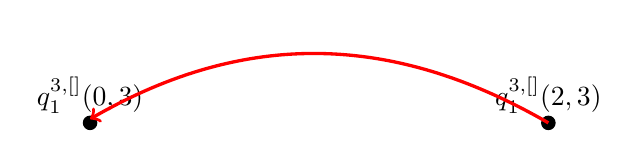
\begin{tikzpicture}[scale=\textwidth/25cm,samples=200]
%%% The nodes represents the k query in the first round
\filldraw[black] (0, 4) circle (5pt) node [anchor=south]{$q^{3, []}_{1}(0, 3)$};
\filldraw[black] (12, 4) circle (5pt) node [anchor=south]{$q^{3, []}_{1}(2, 3)$};
\draw[very thick, ->, red] (12, 4)  to [out=150,in=30] (0, 4.1) ;
\end{tikzpicture}
    \caption{A query-based dependency graph for multi round algorithm}
    \label{fig:multi-round-graph}
\end{figure}
% \begin{figure}
% \begin{tikzpicture}[scale=\textwidth/25cm,samples=200]
% %%% The nodes represents the k query in the first round
% \filldraw[black] (0, 4) circle (5pt) node [anchor=south]{$q^{3, []}_{1}(0, 3)$};
% \filldraw[black] (6, 3) circle (5pt) node [anchor=north]{$q^{3, []}_{1}(1, 3)$};
% \filldraw[black] (12, 4) circle (5pt) node [anchor=south]{$q^{3, []}_{1}(2, 3)$};
% \filldraw[black] (6, 0) circle (5pt) node [anchor=north]{$q^{6, []}_{2}([1, 0, 1])$};
% \draw[very thick, ->, blue] (12, 4)  to [out=150,in=30] (0, 4.1) ;
% % \draw[very thick,->] (3, 4)  -- (0, 4) ;
% % \draw[very thick,->] (0, 0)  -- (6, 2) ;
% %%%%%% The edges represents their dependency relations GROUP 2
% %
% \draw[very thick,->, red]  (12, 4) to [out=150,in=60] (6.1, 3) ;
% \draw[very thick,->, red] (6, 3)  to [out=120,in=30] (0, 3.95) ;
% % %
% %%%%%% The edges represents their dependency relations GROUP 4
% % \draw[very thick,->] (0, 0)  -- (6, 2) ;
% % \draw[very thick,->] (12, 2)  -- (8.1, 2) ;
% \draw[very thick,->, blue] (6, 0)  -- (6, 2.9) ;
% \draw[very thick,->, red] (6, 0)  -- (12, 3.9) ;
% \draw[very thick,->, blue] (6, 0)  -- (0, 3.9) ;
% \end{tikzpicture}
%     \caption{A query-based dependency graph for multi round algorithm}
%     \label{fig:multi-round-graph}
% \end{figure}
%
%
Using \THESYSTEM, we first generate a global list $G$ from an empty list $[]$ and empty whlemap $\emptyset$.
 \[[]; \emptyset; MR^{ssa} \to G; w  \land w = \emptyset\].
 \[G_{k=2} = \left[
  {I_1}^{(1,\emptyset)} , {I_3}^{(2,[2:1])} , {p_1}^{(3,[2:1])} , {a_1}^{(4,[2:1])} ,{I_2}^{(5,[2:1])} ,  {I_3}^{(2,[2:2])} , {p_1}^{(3,[2:2])} , {a_1}^{(4,[2:2])} ,{I_2}^{(5,[2:2])} , {I_3}^{(2,\emptyset)}   \right] \]
  We denote $I_1^{1}$ short for ${I_1}^{(1,\emptyset)}$ and ${I_3}^{(2,1)}$ short for ${I_3}^{(2,[2:1])}$, where the label $(2, 1)$ represents at line number $2$ and in the $1$ st iteration. 
\[
M =  \left[ \begin{matrix}
  I_1^{1} & I_3^{(2,1)} & p_1^{(3,1)} & a_1^{(4,1)} &I_2^{(5,1)}  & I_3^{(2,2)} & p_1^{(3,2)} & a_1^{(4,2)} & I_2^{(5,2)} & I_3^{2}\\
  0 & 0 & 0 & 0 & 0 & 0 & 0 &0 &0&0  \\
 1 & 0 & 0 & 0 & 0 & 0 & 0&0&0&0\\
 0 & 0 & 0 & 0 & 0 & 0& 0& 0 &0&0\\
 0 & 1 & 0 & 0 & 0 & 0 & 0& 0&0&0\\
 0 & 1 & 1 & 1 & 0 & 0 & 0 & 0&0 &0\\
 1 & 0 & 0 & 0 & 1 & 0 & 0& 0&0&0\\
 0 & 0 & 0 & 0 & 0 & 0 & 0& 0&0&0\\
 0 & 0 & 0 & 0 & 0 & 1 & 0& 0&0&0\\
 0 & 0 & 0 & 0 & 0 & 1 & 1 & 1 &0 &0\\
1 & 0 & 0 & 0 & 0 & 0 & 0 & 0 &1&0 \\
 \end{matrix} \right] 
~ , V = \left [ \begin{matrix}
I_1^{1} &  0 \\
I_3^{(2,1)} &  0 \\
p_1^{(3,1)} & 0 \\
a_1^{(4,1)} &  1 \\
I_2^{(5,1)} & 0 \\
I_3^{(2,2)} & 0 \\
p_1^{(3,2)} &  0 \\
a_1^{(4,2)} & 1 \\
I_2^{(5,2)} & 0 \\
I_3^{2} & 0 \\
\end{matrix} \right ]
\]
%
%
%
\begin{figure}
\begin{center}
%
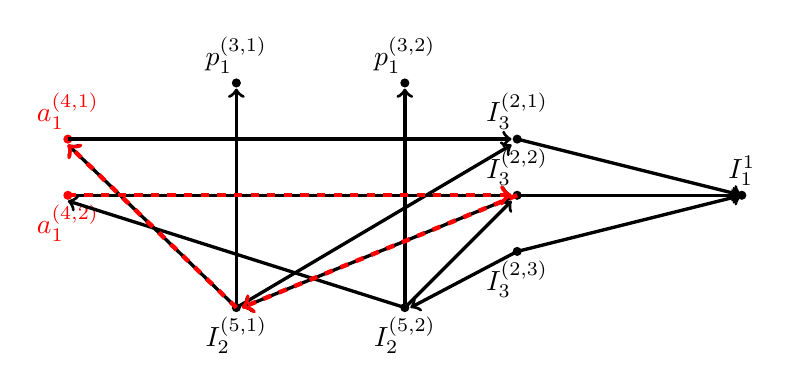
\begin{tikzpicture}[scale=\textwidth/17cm,samples=200]
%%% The nodes represents the k query in the first round
\filldraw[red] (0, 3) circle (2pt) node [anchor=south]{$a_1^{(4,1)}$};
\filldraw[black] (3, 4) circle (2pt) node [anchor=south]{$p_1^{(3,1)}$};
% \filldraw[black] (6, 2) circle (2pt) node [anchor=south]{$q^4_3$};
\filldraw[black] (6, 4) circle (2pt) node [anchor=south]{$p_1^{(3,2)}$};
\filldraw[black] (8, 3) circle (2pt) node [anchor=south]{$I_3^{(2,1)}$};
%%%%%% The nodes represents the n^k queries in the second round
\filldraw[red] (0, 2) circle (2pt) node [anchor=north]{$a_1^{(4,2)}$};
\filldraw[black] (3, 0) circle (2pt) node [anchor=north]{$I_2^{(5,1)}$};
% \filldraw[black] (6, 0) circle (2pt) node [anchor=north]{$q^{3, 7}_{k+1}$};
\filldraw[black] (6, 0) circle (2pt) node [anchor=north]{$I_2^{(5,2)}$};
\filldraw[black] (8, 1) circle (2pt) node [anchor=north]{$I_3^{(2,3)}$};
\filldraw[black] (8, 2) circle (2pt) node [anchor=south]{$I_3^{(2,2)}$};
\filldraw[black] (12, 2) circle (2pt) node [anchor=south]{$I_1^{1}$};
%%%%%The edges between a and I
%%%%% (a1(4,1), I3(2,1))
\draw[very thick, ->] (0, 3)  -- (7.9, 3) ;
%%%%% (a1(4,2), I3(2,2))
\draw[very thick, ->] (0, 2)  -- (7.9, 2) ;
%%%%%% The edges represents their dependency relations GROUP between I3 and I1
\draw[very thick,<-] (12, 2)  -- (8, 2) ;
\draw[very thick,->] (8, 2) -- (3.1, 0) ;
%
\draw[very thick,<-] (12, 2)  -- (8, 1) ;
\draw[very thick,->] (8, 1) -- (6.1, 0) ;
%
\draw[very thick,<-] (12, 2)  -- (8, 3) ;
%
%%%%%% The edges represents their dependency relations GROUP between I2 and others
%%%%%% The edges represents their dependency relations GROUP between I2(5,1) and others
\draw[very thick, ->] (3, 0)  -- (0, 2.9) ;
\draw[very thick, ->] (3, 0)  -- (3, 3.9) ;
\draw[very thick, ->] (3, 0)  -- (7.9, 2.9) ;
%%%%%% The edges represents their dependency relations GROUP between I2(5,2) and others
\draw[very thick, ->] (6, 0)  -- (0, 1.9) ;
\draw[very thick, ->] (6, 0)  -- (6, 3.9) ;
\draw[very thick, ->] (6, 0)  -- (7.9, 1.9) ;
%%%% The longest path representing the adaptivity
\draw[ultra thick, red, ->, dashed] (0, 2) -- (7.9, 2);
\draw[ultra thick, red, ->, dashed] (8, 2) -- (3.1, 0);
\draw[ultra thick, red, ->, dashed] (3, 0)  -- (0, 2.9);
\end{tikzpicture}
\end{center}
    \caption{the variable dependency graph for multi round algorithm}
    \label{fig:multi-round-graph-ssa}
\end{figure}
%
The adaptivity is 1 computed from the graph.
The query-based dependency graph is a subgraph of the variable dependency graph for multi round algorithm.
